\documentclass[10pt,lualatex]{beamer}

\usefonttheme{professionalfonts}
\usepackage{xltxtra}	% XeLaTeX
\usepackage{float}
\usepackage{graphicx}
\usepackage{wrapfig}	% Wrap text around figs
\usepackage{lscape}
\usepackage{rotating}	% Sideways figure
\usepackage{hyperref}	% Hyperlinks
\usepackage{caption}	% Hyperlinks to float top
\usepackage{subcaption}
\usepackage{units}		% dB unit
\usepackage[a4paper,width=150mm,top=25mm,bottom=25mm]{geometry}	% margins
\usepackage{tikz}
\usepackage[section]{placeins}	% Don't let floats float before sections
\usepackage{listings}
\usepackage{amsmath}  % align equations
\usepackage{biblatex}

\usepackage{fancyhdr} % headers-footers
\usepackage{mathtools}
% Tables
\usepackage{array}
\usepackage{booktabs}
% for having numbers aligned to the decimal point
\usepackage{siunitx}


%-------------------------------------Custom commands----------------------------------------------------------
  \usepackage{amsfonts}
  \def \IN{\mathbb N} \def \IZ{\mathbb Z} \def \IQ{\mathbb Q} \def \IR{\mathbb R} \def \IC{\mathbb C}
  \def \NN{\mathbb N} \def \ZZ{\mathbb Z} \def \QQ{\mathbb Q} \def \RR{\mathbb R} \def \CC{\mathbb C}
%-------------------------------GREEK LETTERS DEFINITION-------------------------------------------------------
  \newcommand{\gra}{{\alpha}} \newcommand{\grb}{{\beta}} \newcommand{\grg}{{\gamma}} \newcommand{\grd}{{\delta}}
  \newcommand{\gre}{{\epsilon}} \newcommand{\grz}{{\zeta}} \newcommand{\grh}{{\eta}} \newcommand{\gru}{{\theta}}
  \newcommand{\gri}{{\iota}} \newcommand{\grk}{{\kappa}} \newcommand{\grl}{{\lambda}} \newcommand{\grm}{{\mu}}
  \newcommand{\grn}{{\nu}} \newcommand{\grj}{{\xi}} \newcommand{\gro}{{\rm o}} \newcommand{\grp}{{\pi}}
  \newcommand{\grr}{{\rho}} \newcommand{\grs}{{\sigma}} \newcommand{\grt}{{\tau}} \newcommand{\gry}{{\upsilon}}
  \newcommand{\grf}{{\phi}} \newcommand{\grx}{{\chi}} \newcommand{\grc}{{\psi}} \newcommand{\grv}{{\omega}}
  \newcommand{\grA}{{\rm A}} \newcommand{\grB}{{\rm B}} \newcommand{\grG}{{\Gamma}} \newcommand{\grD}{{\Delta}}
  \newcommand{\grE}{{\rm E}} \newcommand{\grZ}{{\rm Z}} \newcommand{\grH}{{\rm H}} \newcommand{\grU}{{\Theta}}
  \newcommand{\grI}{{\rm I}} \newcommand{\grK}{{\rm K}} \newcommand{\grL}{{\Lambda}} \newcommand{\grM}{{\rm M}}
  \newcommand{\grN}{{\rm N}} \newcommand{\grJ}{{\Xi}} \newcommand{\grO}{{\rm O}} \newcommand{\grP}{{\Pi}}
  \newcommand{\grR}{{\rm R}} \newcommand{\grS}{{\Sigma}} \newcommand{\grT}{{\rm T}} \newcommand{\grY}{{\rm Y}}
  \newcommand{\grF}{{\Phi}} \newcommand{\grX}{{\rm X}} \newcommand{\grC}{{\Psi}} \newcommand{\grV}{{\Omega}}
%---------------------------------------------------------------------------------------------------------------

\setromanfont[Mapping=tex-text]{Linux Libertine O}
\setsansfont[Mapping=tex-text]{DejaVu Sans}
\setmonofont[Mapping=tex-text]{DejaVu Sans Mono}

%\geometry{margin=2.5cm}
\pagestyle{fancy}

\graphicspath{ {figures/} }
\addbibresource{references.bib}

% Alignment and placing of subtables
%   https://tex.stackexchange.com/questions/294589/alignment-and-placing-of-subtables
\usepackage{booktabs,subcaption,amsfonts,dcolumn}
\newcolumntype{d}[1]{D..{#1}}
\newcommand\mc[1]{\multicolumn{1}{c}{#1}} % handy shortcut macro

\renewcommand{\figurename}{Σχήμα}
\renewcommand{\tablename}{Πίνακας}
\renewcommand{\contentsname}{Περιεχόμενα}

\usetikzlibrary{arrows.meta,automata,decorations.pathmorphing,decorations.markings,
  backgrounds,positioning,fit,shapes.misc,
  graphs,arrows
}
\tikzset{node/.style={
    rectangle,
    minimum size= 1.2cm,
    thick, draw=black,
    top color=white!50!yellow!10!,
    bottom color=yellow!50!white!50!,
    font=\ttfamily
}}

\usepackage{fancybox}
\usepackage{minibox}
%\usepackage[backend=biber, style=numeric, citestyle=authoryear]{biblatex}
\usepackage[absolute,overlay]{textpos}
\usetheme{metropolis}
\graphicspath{ {../figures/},{../design_walkthrough/build/} }

\definecolor{light-gray}{gray}{0.22}
\usepackage{../jlcode}
%\lstset{columns=fullflexible,numbersep=0pt,resetmargins= true}

\usepackage{minted}
\usemintedstyle{paraiso-dark}
%\usemintedstyle{lovelace}
%\usemintedstyle{friendly}
\setmonofont{Everson Mono}

\defbeamertemplate{description item}{align left}{\insertdescriptionitem\hfill}

\setbeamercolor{framesource}{fg=gray}
\setbeamerfont{framesource}{size=\tiny}
\newcommand{\source}[1]{\begin{textblock*}{4cm}(0.3cm,8.6cm)
    \begin{beamercolorbox}[ht=0.5cm,left]{framesource}
        \usebeamerfont{framesource}\usebeamercolor[fg]{framesource} Πηγή: {#1}
    \end{beamercolorbox}
\end{textblock*}}


%---		BIBLIOGRAPHY		---%
\bibliography{../references.bib}
%\setbeamertemplate{bibliography item}[text]
\renewcommand*{\bibfont}{\footnotesize}

\newcommand{\titlestring}{Υψηλού επιπέδου υλοποίηση των αλγορίθμων Hierarchical Temporal Memory σε Julia}
\newcommand{\authorstring}{Κωνσταντίνος Σαμαράς-Τσακίρης}
\hypersetup{%
    pdfencoding=auto,
    pdfauthor={\authorstring},
    pdftitle={\titlestring}
    }

\title{\huge{\titlestring}}
\author{\authorstring\\
Επιβλέπων καθηγητής: Νίκος Πιτσιάνης}
\date{13 Ιουνίου 2019}


\begin{document}

\begin{frame}%{\maketitle}
  \titlepage
\end{frame}

\begin{frame}{Νευρώνας}
  \centering
	\begin{figure}[h]
		\begin{subfigure}{0.30\textwidth}
			\includesvg[width=\textwidth]{../figures/pyramidal_cell.svg}
		\end{subfigure}
		\hfill
		\begin{subfigure}{0.65\textwidth}
			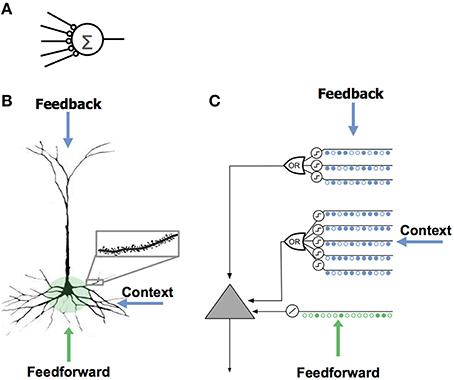
\includegraphics[width=\textwidth]{../figures/numenta_neuron}
		\end{subfigure}
	\end{figure}
\end{frame}

\begin{frame}{Μικροστήλες}
  \centering
  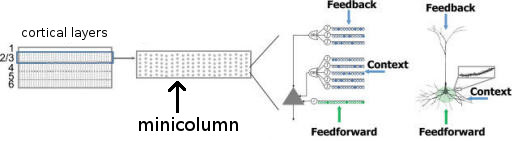
\includegraphics[width=\textwidth]{../figures/layer-minicolumn}
\end{frame}

\begin{frame}{Φλοιικές στήλες}
  \centering
  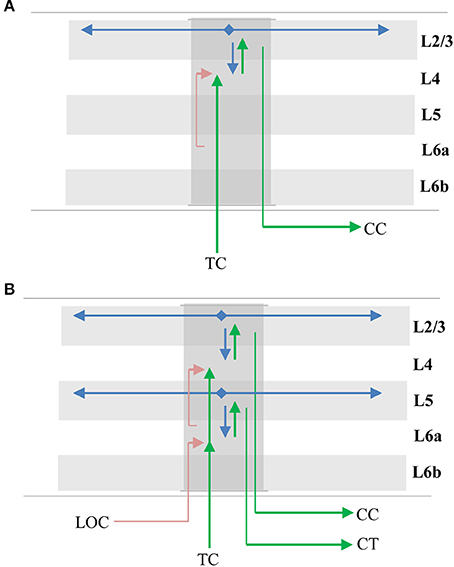
\includegraphics[width=.6\textwidth]{../figures/layers_in_column}
\end{frame}

\begin{frame}{Αναστολή μεταξύ μικροστηλών}
  \centering
  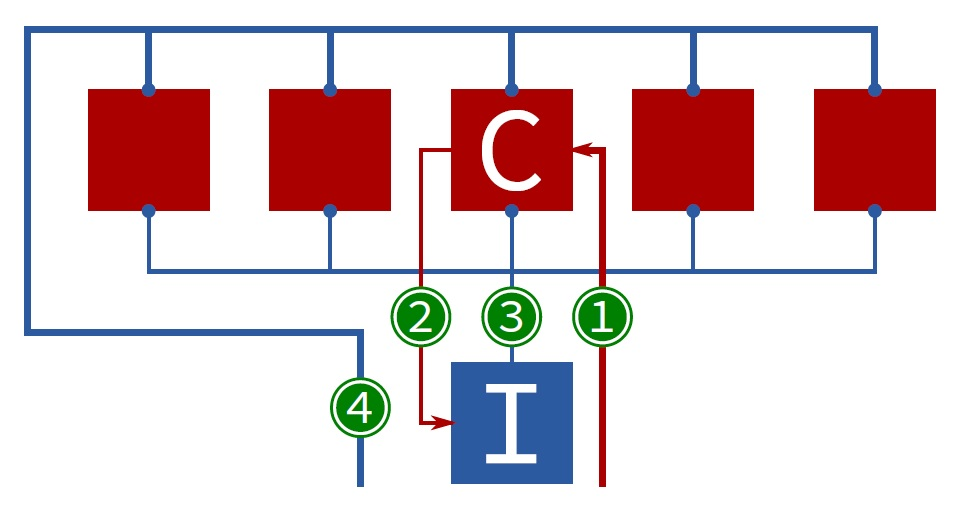
\includegraphics[width=\textwidth]{../figures/spatial_hardware}
\end{frame}

\begin{frame}{Χωρικός συγκεντρωτής}
  \centering
  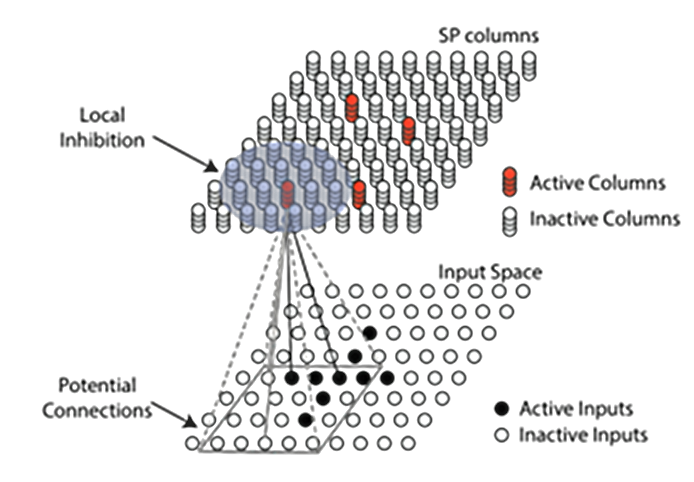
\includegraphics[width=.9\textwidth]{../figures/vlsi-present/spatpool}
\end{frame}

\section{Στοιχεία Χωρικού Συγκεντρωτή}
\begin{frame}[fragile]{Τοπολογία εισόδου/εξόδου: υπερκύβος}
  \begin{block}{Δείκτης υπερκύβου}
    \[ I(x_j; x_i^c, γ) = \mathit{true} \iff x_j \in \text{ hypercube} \]
    \begin{itemize}
      \item[] $x^c$: κέντρο υπερκύβου
      \item[] $γ$: ακτίνα υπερκύβου
    \end{itemize}
  \end{block}
  \begin{block}{Εν δυνάμει συνδέσεις}
    \[ Π_i= \{j \;|\, I(x_j; x_i^c, γ) \wedge Z_{ij} < p\} \]
    όπου $Ζ \in U(0,1)$ τυχαίος αριθμός
  \end{block}
\end{frame}

\begin{frame}[fragile]{Τοπολογία εισόδου/εξόδου: υπερκύβος}
\begin{minted}[fontsize=\scriptsize,bgcolor=light-gray,breaklines]{julia}
struct Hypercube{N}
  xᶜ::NTuple{N,Int}
  γ::Int
  sz::NTuple{N,Int}
  indices::CartesianIndices{N}
end
Hypercube(xᶜ,γ,sz)= Hypercube(xᶜ,γ,sz, start(xᶜ,γ,sz))
start(xᶜ,γ,sz)= CartesianIndices(map( (a,b)-> a:b,
                    max.(xᶜ .- γ, 1),
                    min.(xᶜ .+ γ, sz) ))
Base.collect(hc::Hypercube)= map(c->c.I, collect(hc.indices))

jl> collect(Hypercube((1,1),1,(5,5)))
2×2 Array{Tuple{Int64,Int64},2}:
 (1, 1)  (1, 2)
 (2, 1)  (2, 2)
\end{minted}
\end{frame}


\section{Βιβλιογραφία}
%\nocite{*}
\begin{frame}[plain,allowframebreaks]
  \printbibliography
\end{frame}

\end{document}
